% Provenance (never printed): see sources/outline_sources.md (Year 1: physical and chemical
% weathering; hydrolysis and its degrees; the ionic-potential diagram; clay minerals and
% climate; silicate weathering and carbon dioxide). Exercise and problem values in the Book 3
% scratch calculator calc/ch19.py; figure data from figdata/bachelor-1/ionic_potential.py and
% hydrolysis.py. Weathering is owned by Book 1 g5; chemical weathering, hydrolysis, clay mineral
% and laterite by Book 2 g10 (re-founded here). Silicate classes and the feldspars by ch. 7;
% Bowen's series by Book 2 g11; acid--base chemistry, solubility and oxidation by the chemistry
% books; soils and their horizons by the biology books. The silicate-weathering thermostat
% belongs to the Year 2 volume (told).
\chapter{अपक्षय और मृत्तिकाएँ}\label{ch:b1:weathering-clays}

एक पुरानी कब्र-पट्टिका के अक्षर धुँधले पड़ते हैं, उनके तीखे किनारे उथली खाँचों में गोल होते जाते हैं, संगमरमर की पट्टिका पर स्लेट की तुलना में तेज़ी से। एक ग्रेनाइट का उद्भेद, जो पृथ्वी पर किसी भी चीज़ जितना कठोर दिखता है, अपनी सतह पर किरकिरी बालू में टूट जाता है, जो उँगलियों के बीच से काँच जैसे क्वार्ट्ज, चॉक-जैसे फ़ेल्डस्पार और \omterm{def:b1:rock-forming-minerals:groups}{अभ्रक} के पत्रों के ढीले कणों की तरह बहती है। आर्द्र उष्णकटिबंधीय के जंगलों के नीचे ठोस चट्टान गहराई में पड़ी हो सकती है, एक लाल मिट्टी के नीचे, जो चट्टान के खनिजों की रूपरेखा रखती है पर उसे फावड़े से काटा जा सकता है। तीनों पानी के काम हैं, पृथ्वी की सतह पर। यह अध्याय उस काम को रसायन-विज्ञान के रूप में लिखता है: कौन-से \omterm{def:b1:rock-forming-minerals:mineral}{खनिज} पहले झुकते हैं, वे क्या बन जाते हैं, क्यों कुछ तत्व पानी के साथ निकल जाते हैं और अन्य रुकते हैं, जलवायु परिणाम कैसे तय करती है, और सिलिकेट चट्टान का धीमा क्षय हवा से कार्बन डाइऑक्साइड कैसे खींचता है।

\begin{recall}
अपक्षय चट्टानों को वहीं तोड़ता है जहाँ वे पड़ी हैं (पुस्तक~1, कक्षा~5)। \omterm{def:b1:weathering-clays:weathering}{रासायनिक अपक्षय} खनिजों को रूपांतरित करता है; फ़ेल्डस्पार का \omterm{def:b1:weathering-clays:hydrolysis}{जल-अपघटन} एक \omterm{def:b1:weathering-clays:clay-mineral}{मृत्तिका-खनिज}, \omterm{def:b1:weathering-clays:clay-mineral}{कैओलिनाइट}, देता है और पोटैशियम तथा सिलिका को नदियों में भेजता है; \omterm{def:b1:weathering-clays:laterite}{लैटेराइट} गर्म, आर्द्र जलवायु का लौह- और ऐल्युमिनियम-समृद्ध, लाल उत्पाद है (पुस्तक~2, कक्षा~10)। सिलिकेटों का वर्गीकरण इस पर होता है कि उनके \ce{SiO4} चतुष्फलक कोने कैसे साझा करते हैं: \omterm{def:b1:rock-forming-minerals:silicate-classes}{फ़िलोसिलिकेट} परतें बनाते हैं; फ़ेल्डस्पार सोडियम, पोटैशियम और कैल्शियम के ढाँचा-सिलिकेट हैं, और \omterm{def:b1:rock-forming-minerals:groups}{अभ्रक} पत्र-सिलिकेट हैं जिनकी परतों के बीच पोटैशियम होता है (\cref{def:b1:rock-forming-minerals:silicate-classes}, \cref{def:b1:rock-forming-minerals:groups})। किसी आयन की आयनिक त्रिज्या उसके आवेश और उसके समन्वय पर निर्भर करती है (\cref{ch:b1:rock-forming-minerals})। \omterm{def:b1:rock-forming-minerals:mineral}{खनिज} एक ठंडे होते मैग्मा से बोवेन की अभिक्रिया-श्रेणी के क्रम में जमते हैं, \omterm{def:b1:rock-forming-minerals:groups}{ओलिवीन} पहले और क्वार्ट्ज अंत में (पुस्तक~2, कक्षा~11)। अम्ल हाइड्रोजन आयन छोड़ता है; पानी में घुली कार्बन डाइऑक्साइड कार्बोनिक अम्ल बनाती है; ऑक्सीकरण इलेक्ट्रॉनों की हानि है; एक संतुलित समीकरण हर तत्व और आवेश को संरक्षित रखता है (रसायन-विज्ञान की पुस्तकें)। मिट्टी एक जीवित परत है जो क्षितिजों में संगठित है (जीव-विज्ञान की पुस्तकें)।
\end{recall}

\section{भौतिक और रासायनिक अपक्षय}\label{sec:b1:weathering-clays:types}

पृथ्वी की गहराई में, ऊँचे ताप और दाब पर, और मुक्त जल या ऑक्सीजन के बिना बनी चट्टान, सतह पर साम्यावस्था से बाहर है। वह दो तरीकों से समायोजित होती है, जो साथ-साथ काम करते हैं।

\begin{definition}[भौतिक अपक्षय, रासायनिक अपक्षय]
\label{def:b1:weathering-clays:weathering}
\emph{भौतिक अपक्षय}\index{भौतिक अपक्षय} एक चट्टान का अपने स्थान पर उसके खनिजों में बिना परिवर्तन के छोटे टुकड़ों में टूटना है। \emph{रासायनिक अपक्षय}\index{रासायनिक अपक्षय} एक चट्टान के खनिजों का अपने स्थान पर जल और उसके साथ ले जाए गए पदार्थों के साथ अभिक्रिया द्वारा रूपांतरण है, मुख्यतः हाइड्रोजन आयनों, घुली कार्बन डाइऑक्साइड और ऑक्सीजन के साथ: कुछ \omterm{def:b1:rock-forming-minerals:mineral}{खनिज} घुल जाते हैं, अन्य सतह पर स्थायी नए खनिजों से प्रतिस्थापित होते हैं, और चट्टान का एक भाग विलयन में निकल जाता है।
\end{definition}
% ledger: formoso:weathering

\emph{पाला।} शून्य \qty{0}{\celsius} पर जल का घनत्व \qty{999.87}{kg.m^{-3}} है, बर्फ़ का \qty{916.72}{kg.m^{-3}}: जल जमने पर \qty{9.1}{\percent} फैलता है। पाले के अपक्षय का पुराना चित्र यह है कि एक बंद दरार में जमता जल उसे खोल देता है, हर पिघलने और जमने पर फिर से। ग्रेनाइट और संगमरमर की दरारों का एक प्रतिरूप, जो भंजन यांत्रिकी और जमती मिट्टियों के ज्ञात तथ्यों पर बना है, भार कहीं और रखता है: पानी छिद्रों से होकर उस बर्फ़ की ओर खिंचता है जो पहले से दरार में है, जैसे वह जमती मिट्टी की बर्फ़-परतों की ओर खिंचता है, और बर्फ़ तब तक बढ़कर दरार को पच्चर से खोलती है जब तक जमाव चलता है। लगातार जमाव लगभग \qty{-4}{\celsius} और \qty{-15}{\celsius} के बीच सबसे प्रभावी है: शून्य के निकट बर्फ़ पर्याप्त दाब नहीं बना सकती, और ठंडे तापमान पर पानी उस तक नहीं जा सकता।
% ledger: usgs:water-density, iapws:ice-density, wh85:frost

\emph{ताप, भार-मोचन और लवण।} बार-बार गर्म होना और ठंडा होना उस चट्टान को थका देता है जिसके \omterm{def:b1:rock-forming-minerals:mineral}{खनिज} अलग-अलग मात्रा में फैलते हैं; अपरदन द्वारा सतह पर लाया गया ग्रेनाइट, अपने ऊपर के भार से मुक्त होकर, फैलता है और सतह के समांतर चादरों में फट जाता है; वाष्पित होते पानी से जमते लवण, मरुस्थलों और तटों पर, कणों को अलग कर देते हैं।

\omterm{def:b1:weathering-clays:weathering}{भौतिक अपक्षय} केवल चट्टान नहीं तोड़ता: वह उसे पानी के लिए खोलता है।

\begin{proposition}[खंडन से खुली सतह]\label{prop:b1:weathering-clays:surface}
लंबाई $L$ के घन को लंबाई $L/n$ के घनों में काटने पर $n$ गुना सतह-क्षेत्रफल मिलता है। अधिक सामान्यतः, द्रव्यमान $m$ के कणों का, घनत्व $\rho$ के, सब लंबाई $d$ के घन, सतह-क्षेत्रफल $S = 6m/(\rho d)$ रखता है: विशिष्ट सतह $S/m =
6/(\rho d)$ कण-आकार के व्युत्क्रमानुपाती है।
\end{proposition}

\begin{proof}
लंबाई $d$ के घन का क्षेत्रफल $6d^2$ और द्रव्यमान $\rho d^3$ है, इसलिए हर कण की, और उनकी किसी भी संख्या की, विशिष्ट सतह $6d^2/(\rho d^3)
= 6/(\rho d)$ है। लंबाई $L$ के घन को $n^3$ घनों में, लंबाई $L/n$ के, काटने से द्रव्यमान वही रहता है और $d$ का $n$ से भाग होता है, जो क्षेत्रफल को $n$ गुना करता है।
\end{proof}

घनत्व लगभग \qty{2600}{kg.m^{-3}} के फ़ेल्डस्पार के एक खंड की विशिष्ट सतह \qty{0.23}{m^2.kg^{-1}} है जब वह सेंटीमीटर के टुकड़ों में हो, और \qty{2.3}{m^2.g^{-1}} जब वह माइक्रोमीटर के कणों में हो, दस हज़ार गुना अधिक। रासायनिक अभिक्रियाएँ सतहों पर होती हैं, इसलिए पाले से चूर-चूर या अपने जोड़ों पर खुली चट्टान, अक्षुण्ण उसी चट्टान की तुलना में कहीं तेज़ी से रासायनिक रूप से अपक्षयित होती है।
% ledger: hom:albite, hom:orthoclase

\emph{रासायनिक अभिक्रियाएँ।} कैल्साइट कार्बन डाइऑक्साइड वाले पानी में पूरी तरह घुल जाता है, इसीलिए संगमरमर की कब्र-पट्टिकाएँ अपने अक्षर खोती हैं (पुस्तक~2, कक्षा~10)। गहरे सिलिकेटों का आयरन(II) आयरन(III) तक ऑक्सीकृत होता है, जो पीले-भूरे और लाल ऑक्साइडों के रूप में रहता है। सबसे महत्वपूर्ण, क्योंकि सिलिकेट \omterm{def:b1:layered-earth:layers}{भूपर्पटी} के अधिकांश भाग बनाते हैं, \omterm{def:b1:weathering-clays:hydrolysis}{जल-अपघटन} है। हाइड्रोजन आयन कार्बन डाइऑक्साइड से आते हैं, जो हवा से घुलती है और जड़ों तथा अपघटकों द्वारा मिट्टी में छोड़ी जाती है, और सड़ते पौधों के कार्बनिक अम्लों से: अप्रदूषित सतही और मिट्टी के जल का pH 5.5 और 7 के बीच है, और कुछ वन-मिट्टियों की कार्बनिक परत का जल \num{3.5} तक नीचे। जल, ताप, सतह-क्षेत्रफल और अम्लता इस प्रकार \omterm{def:b1:weathering-clays:weathering}{रासायनिक अपक्षय} के चार नियंत्रक हैं, और एक गर्म, आर्द्र जलवायु जिसमें मोटी मिट्टी हो, ये चारों देती है।
% ledger: formoso:weathering

\section{सिलिकेटों का जल-अपघटन}\label{sec:b1:weathering-clays:hydrolysis}

\begin{definition}[सिलिकेट का जल-अपघटन]
\label{def:b1:weathering-clays:hydrolysis}
एक सिलिकेट का \emph{जल-अपघटन}\index{जल-अपघटन (सिलिकेटों का)} उसकी जल और हाइड्रोजन आयनों के साथ वह अभिक्रिया है जिसमें हाइड्रोजन आयन धातु धनायनों का स्थान लेते हैं, जो विलयन में चले जाते हैं; सिलिकॉन का भाग या सारा घुले सिलिसिक अम्ल \ce{H4SiO4} के रूप में निकलता है, और \omterm{def:b1:rock-forming-minerals:mineral}{खनिज} का शेष एक नए ठोस में पुनर्निर्मित होता है, एक \omterm{def:b1:weathering-clays:clay-mineral}{मृत्तिका-खनिज} या एक हाइड्रॉक्साइड। यह विलयन असंगत है: बचा ठोस उस \omterm{def:b1:rock-forming-minerals:mineral}{खनिज} का संघटन नहीं रखता जिस पर हमला हुआ।
\end{definition}
% ledger: formoso:weathering

अभिक्रिया लिखने की कुंजी ऐल्युमिनियम है: मिट्टियों और नदियों के pH पर वह लगभग अघुलनशील है, और ठोस उत्पाद उसे सब रखता है। बाकी सब उसी से निकलता है।

\begin{method}[जल-अपघटन अभिक्रिया का संतुलन]
\label{met:b1:weathering-clays:balance}
हमला हुए \omterm{def:b1:rock-forming-minerals:mineral}{खनिज} और ठोस उत्पाद दिए होने पर:
\begin{enumerate}
  \item उत्पाद का एक सूत्र-एकक लीजिए, और \omterm{def:b1:rock-forming-minerals:mineral}{खनिज} की उतनी मात्रा जो उतने ही ऐल्युमिनियम परमाणु लाए।
  \item \omterm{def:b1:rock-forming-minerals:mineral}{खनिज} का सिलिकॉन जो उत्पाद द्वारा प्रयुक्त नहीं हुआ, \ce{H4SiO4} के रूप में निकलता है; धातु धनायन जो उत्पाद द्वारा प्रयुक्त नहीं हुए, आयनों के रूप में निकलते हैं।
  \item इन धनायनों के आवेश को बाईं ओर हाइड्रोजन आयनों से संतुलित कीजिए।
  \item ऑक्सीजन को बाईं ओर जल से संतुलित कीजिए।
  \item हाइड्रोजन जाँचिए: उसे अपने आप संतुलित होना चाहिए। यदि नहीं होता, तो एक सूत्र गलत है।
  \item यदि पूर्ण-संख्या का समीकरण चाहिए, तो सबको गुणा कीजिए।
\end{enumerate}
\end{method}

\begin{proposition}[फ़ेल्डस्पारों का जल-अपघटन]\label{prop:b1:weathering-clays:feldspars}
\omterm{def:b1:weathering-clays:clay-mineral}{स्मेक्टाइट} बेइडेलाइट \ce{Na_{0.5}Al2(Si_{3.5}Al_{0.5})O10(OH)2} (अंतर-परत जल छोड़कर), \omterm{def:b1:weathering-clays:clay-mineral}{कैओलिनाइट} \ce{Al2Si2O5(OH)4} और गिब्साइट \ce{Al(OH)3} उत्पादों के रूप में लेने पर,
\begin{align*}
&\ce{5 NaAlSi3O8 + 4 H+ + 16 H2O -> 2 Na_{0.5}Al2(Si_{3.5}Al_{0.5})O10(OH)2 + 4 Na+ + 8 H4SiO4},\\ % ce-unbalanced-ok: decimal subscripts the checker cannot read; balance tested in tests/bachelor-1/test_weathering_clays.py
&\ce{2 NaAlSi3O8 + 2 H+ + 9 H2O -> Al2Si2O5(OH)4 + 2 Na+ + 4 H4SiO4},\\
&\ce{NaAlSi3O8 + H+ + 7 H2O -> Al(OH)3 + Na+ + 3 H4SiO4},\\
&\ce{CaAl2Si2O8 + 2 H+ + H2O -> Al2Si2O5(OH)4 + Ca^2+}.
\end{align*}
एल्बाइट पहली अभिक्रिया में अपने सोडियम का \qty{80}{\percent} और अपने सिलिकॉन का $8/15$ विलयन में खोता है, दूसरी में अपना सारा सोडियम और अपने सिलिकॉन का $2/3$, और तीसरी में दोनों का सब। एनॉर्थाइट अपना सारा कैल्शियम खोता है और अपना कोई सिलिकॉन नहीं।
\end{proposition}
% ledger: webmineral:clays-b19, hom:albite, hom:anorthite

\begin{proof}
मान लीजिए: विधि लागू कीजिए। पहली अभिक्रिया: दो बेइडेलाइट इकाइयों में $2\times2.5 = 5$ ऐल्युमिनियम है, 5 एल्बाइट का ऐल्युमिनियम; एल्बाइट के 15 सिलिकॉन, घटे उत्पाद के $2\times3.5 = 7$, 8 \ce{H4SiO4} छोड़ते हैं; 5 सोडियम घटे 1, 4 \ce{Na+} छोड़ते हैं, 4 \ce{H+} से संतुलित; ऑक्सीजन, बाईं ओर $40 + w$ और दाईं ओर $24 + 32 =
56$, $w = 16$ देता है; हाइड्रोजन, $4 + 32 = 36$ और $4 + 32 = 36$, जाँचा गया। दूसरी: 2 एल्बाइट \omterm{def:b1:weathering-clays:clay-mineral}{कैओलिनाइट} के 2 ऐल्युमिनियम देते हैं, $6 - 2 = 4$ \ce{H4SiO4}, 2 \ce{Na+} और 2 \ce{H+}; ऑक्सीजन $16 + w = 9 + 16$ से $w = 9$; हाइड्रोजन $2 + 18 = 20 = 4 + 16$। तीसरी: एक एल्बाइट, तीन सिलिसिक अम्ल, एक \ce{Na+} और एक \ce{H+}; ऑक्सीजन $8 + w = 3 + 12$ से $w = 7$; हाइड्रोजन $1 + 14 = 15 = 3 + 12$। चौथी: एनॉर्थाइट के 2 ऐल्युमिनियम और 2 सिलिकॉन ठीक \omterm{def:b1:weathering-clays:clay-mineral}{कैओलिनाइट} के हैं, कोई सिलिसिक अम्ल नहीं निकलता, \ce{Ca^2+} को 2 \ce{H+} चाहिए; ऑक्सीजन $8 + w = 9$ से $w = 1$; हाइड्रोजन $2 + 2 = 4$। निर्यातित भाग वे आयन हैं जो विलयन में हैं, \omterm{def:b1:rock-forming-minerals:mineral}{खनिज} के परमाणुओं के ऊपर: $4/5$ और $8/15$, फिर $2/2$ और $4/6$, फिर $1/1$ और $3/3$।
\end{proof}

वही एल्बाइट तीन भिन्न ठोस दे सकता है, और कौन-सा देता है यह इस पर निर्भर है कि कितना पानी चट्टान से होकर गुज़रता है और उत्पादों को बहा ले जाता है: थोड़ा पानी, तो सिलिका का बहुत-सा भाग और कुछ धनायन एक \omterm{def:b1:weathering-clays:clay-mineral}{स्मेक्टाइट} बनाने के लिए रुकते हैं; अधिक, तो केवल \omterm{def:b1:weathering-clays:clay-mineral}{कैओलिनाइट} के लिए पर्याप्त सिलिका रुकती है; बहुत अधिक, तो सिलिका पूरी तरह निकल जाती है।

\begin{definition}[द्वि-सिऐलिटीकरण, एक-सिऐलिटीकरण, ऐलिटीकरण]\label{def:b1:weathering-clays:hydrolysis-degree}
सिलिकेटों के \omterm{def:b1:weathering-clays:hydrolysis}{जल-अपघटन} की मात्रा उसके उत्पाद से नामित होती है। \emph{द्वि-सिऐलिटीकरण}\index{द्वि-सिऐलिटीकरण} 2:1 \omterm{def:b1:weathering-clays:clay-mineral}{मृत्तिका-खनिज} बनाता है, जैसे \omterm{def:b1:weathering-clays:clay-mineral}{स्मेक्टाइट}, जिनमें हर ऐल्युमिनियम परमाणु पर लगभग दो सिलिकॉन परमाणु हैं; धनायनों का एक भाग उनमें रहता है। \emph{एक-सिऐलिटीकरण}\index{एक-सिऐलिटीकरण} 1:1 \omterm{def:b1:weathering-clays:clay-mineral}{मृत्तिका-खनिज} बनाता है, \omterm{def:b1:weathering-clays:clay-mineral}{कैओलिनाइट}, जिसमें हर ऐल्युमिनियम पर एक सिलिकॉन है; सारे क्षारीय और क्षारीय-मृदा धनायन निकल जाते हैं। \emph{ऐलिटीकरण}\index{ऐलिटीकरण} सिलिकॉन को पूरी तरह हटाता है और ऐल्युमिनियम हाइड्रॉक्साइड, गिब्साइट, छोड़ता है।
\end{definition}
% ledger: pedron:stages, formoso:weathering

पहुँची मात्रा पहले जलवायु पर निर्भर करती है, वर्षा और ताप के माध्यम से, और फिर परिच्छेद की निकास-व्यवस्था पर। जहाँ पानी का नवीकरण कम होता है, एक ग्रेनाइट अपने सोडियम और कैल्शियम का बहुत-सा भाग खोता है, पोटैशियम धीमे, और अपने सिलिका का केवल एक हिस्सा: उसके फ़ेल्डस्पार 2:1 मृत्तिकाओं में बदलते हैं, और बहुत-सा क्वार्ट्ज बचा रहता है; चट्टान एक ऐसी बालू में टूट जाती है जिसमें क्वार्ट्ज, \omterm{def:b1:rock-forming-minerals:groups}{अभ्रक} और आधा-अपक्षयित फ़ेल्डस्पार मृत्तिका के साथ मिले हों। आर्द्र उष्णकटिबंधीय की भारी वर्षा के नीचे, प्रति वर्ष \qty{2000}{mm} से अधिक, धनायन और सिलिका कहीं अधिक निक्षालित होते हैं, और \omterm{def:b1:weathering-clays:clay-mineral}{कैओलिनाइट}, Si/Al = 1, बनता है। जहाँ निक्षालन सबसे प्रबल है, वहाँ \omterm{def:b1:weathering-clays:clay-mineral}{कैओलिनाइट} का सिलिका भी चला जाता है, और गिब्साइट बचता है।
% ledger: pedron:stages, goldich:1938, formoso:laterite

\begin{omfigure}
\begin{tikzpicture}[font=\small]
% fractions of albite's Na and Si exported by the three degrees (figdata/bachelor-1/hydrolysis.py)
\begin{axis}[width=10.5cm, height=6cm, ybar, bar width=0.5cm, ymin=0, ymax=112,
    xmin=0.45, xmax=3.55, xtick={1,2,3},
    xticklabels={{द्वि-सिऐलिटीकरण\\ से बेइडेलाइट\\ (Si/Al = 1.4)}, {एक-सिऐलिटीकरण\\ से कैओलिनाइट\\ (Si/Al = 1)}, {ऐलिटीकरण\\ से गिब्साइट\\ (Si/Al = 0)}},
    xticklabel style={align=center, font=\footnotesize},
    ylabel={विलयन में निर्यात (\si{\percent})}, ytick={0,20,...,100},
    legend style={at={(0.5,1.03)}, anchor=south, font=\footnotesize, legend columns=2, draw=none},
    nodes near coords={\pgfmathprintnumber[fixed,precision=0]{\pgfplotspointmeta}}, every node near coord/.append style={font=\scriptsize},
    enlarge x limits=false]
  \addplot[fill=omThm!60, draw=omThm!80!black] table[x=degree, y=Na] {figdata/out/bachelor-1-hydrolysis-degrees.dat};
  \addplot[fill=omDef!55, draw=omDef!80!black] table[x=degree, y=Si] {figdata/out/bachelor-1-hydrolysis-degrees.dat};
  \legend{सोडियम, सिलिकॉन}
\end{axis}
\end{tikzpicture}

{\small एल्बाइट के \omterm{def:b1:weathering-clays:hydrolysis}{जल-अपघटन} की तीन मात्राएँ: उसके सोडियम और सिलिकॉन का कितना प्रतिशत विलयन में बहा, संतुलित अभिक्रियाओं से परिकलित, और बचे ठोस का सिलिकॉन-से-ऐल्युमिनियम अनुपात। ऐल्युमिनियम तीनों में पूरी तरह ठोस में रहता है।}
\label{fig:b1:weathering-clays:degrees}
\end{omfigure}


\begin{omfigure}
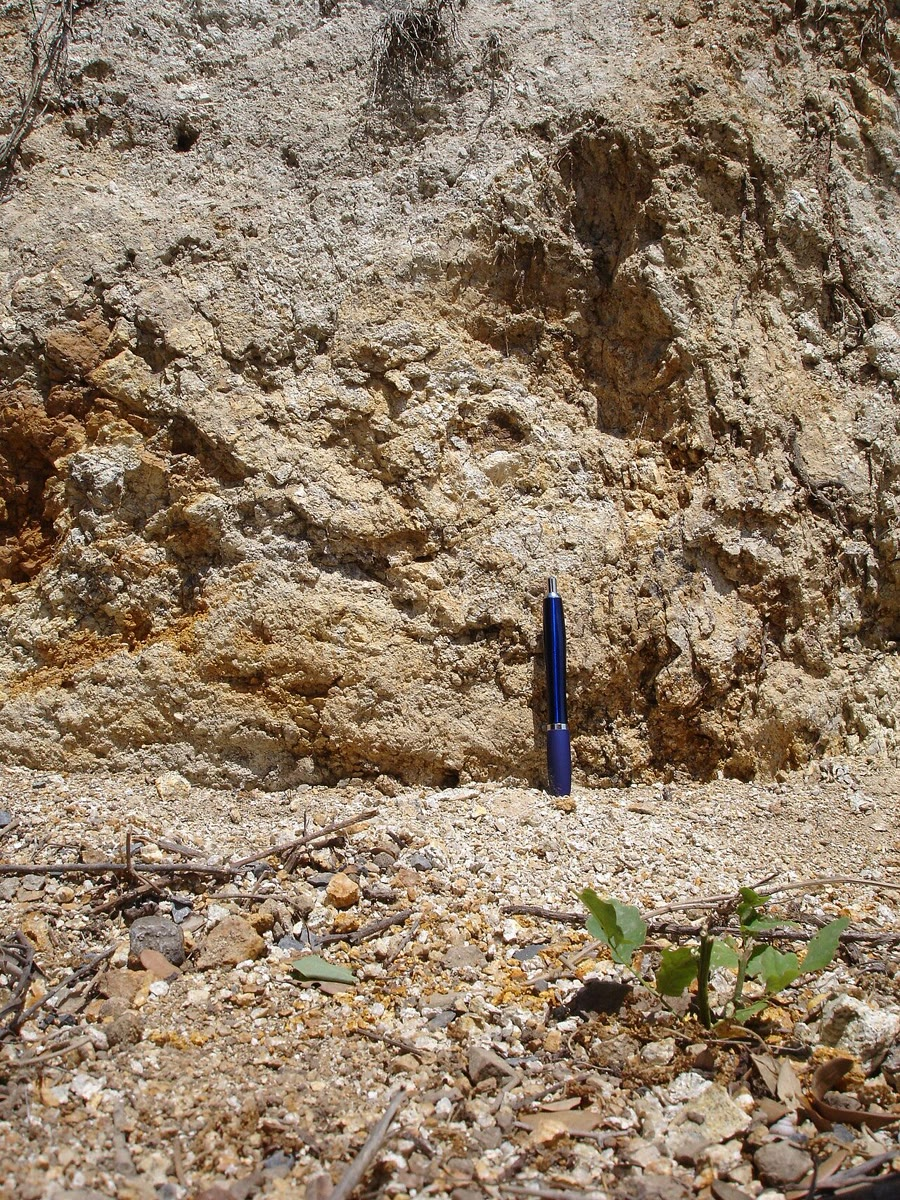
\includegraphics[height=6.3cm]{images/book3/b1-granite-grus.jpg}\hfill
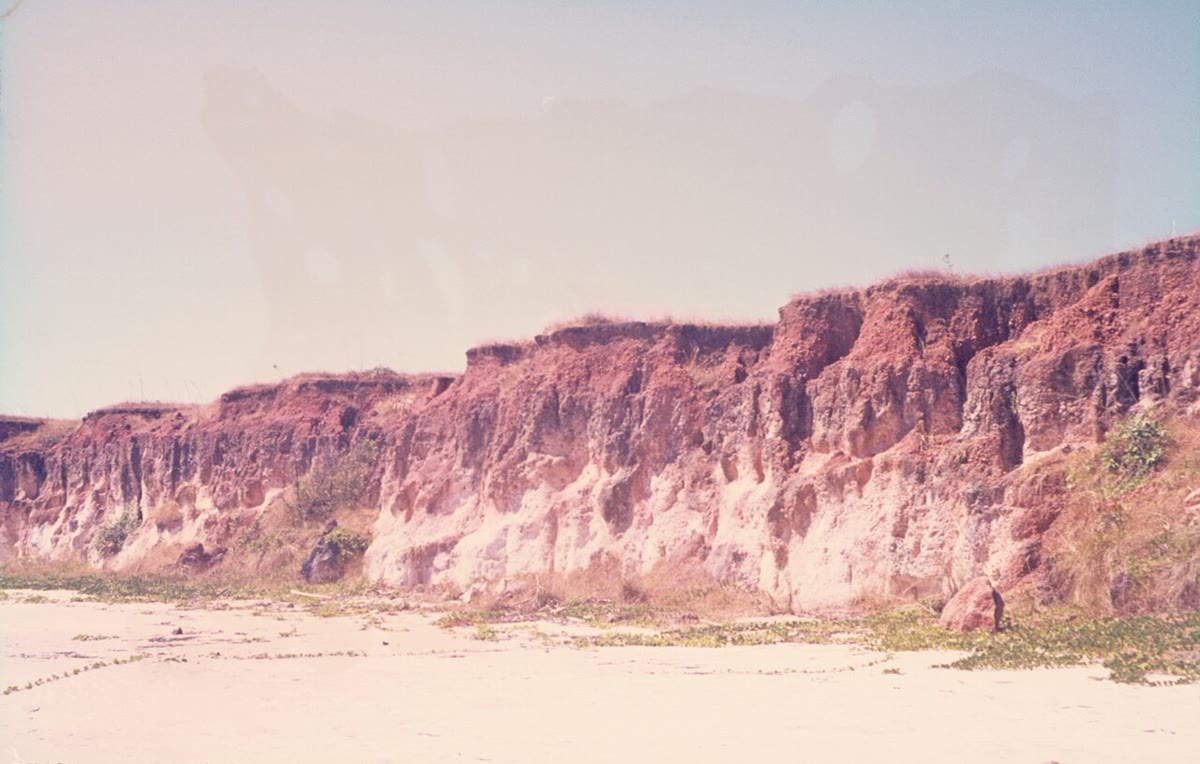
\includegraphics[height=6.3cm]{images/book3/b1-bauxite-weipa.jpg}
{\small बाएँ: पिरेनीज़ में सड़ा ग्रेनाइट, जो अब भी अपनी जगह पर है, पर क्वार्ट्ज, फ़ेल्डस्पार और \omterm{def:b1:rock-forming-minerals:groups}{अभ्रक} की बालू में टूटता हुआ है, और उसके पैर में ढीली बालू पड़ी है; पैमाना पेन से दिया गया है। फ़ोटो: Pinpin, CC~BY~2.5। दाएँ: उत्तरी ऑस्ट्रेलिया में वेइपा के तट पर एक अपक्षय-परिच्छेद: लाल बॉक्साइट, जो \omterm{def:b1:weathering-clays:hydrolysis-degree}{ऐलिटीकरण} का उत्पाद है, एक सफ़ेद कैओलिनाइट-समृद्ध बलुआ पत्थर के ऊपर। फ़ोटो: Werner Schellmann, 1969, CC~BY-SA~2.5। दोनों विकिमीडिया कॉमन्स से।}
\label{fig:b1:weathering-clays:photos}
\end{omfigure}
% ledger: commons:grus, commons:weipa

\emph{कौन-सा \omterm{def:b1:rock-forming-minerals:mineral}{खनिज} पहले जाता है।} 1938 में सैमुअल गोल्डिख ने अपक्षीकृत परिच्छेदों की उनकी जनक-चट्टानों से तुलना करते हुए अपक्षय में कम से अधिक स्थायी खनिजों की एक श्रृंखला प्रस्तावित की, और पाया कि वह उसी क्रम का अनुसरण करती है जिसमें वे एक मैग्मा से जमते हैं: पहले \omterm{def:b1:rock-forming-minerals:groups}{ओलिवीन} और कैल्शियम-समृद्ध \omterm{def:b1:rock-forming-minerals:groups}{प्लैजियोक्लेज़}, अंत में क्वार्ट्ज। सबसे अधिक ताप पर बने \omterm{def:b1:rock-forming-minerals:mineral}{खनिज} सतह की साम्यावस्था से सबसे दूर होते हैं। एक आधुनिक सूची, कम से अधिक प्रतिरोधी की ओर, यह है: पाइराइट, कैल्साइट, डोलोमाइट, \omterm{def:b1:rock-forming-minerals:groups}{ओलिवीन}, कैल्शियम \omterm{def:b1:rock-forming-minerals:groups}{प्लैजियोक्लेज़}, \omterm{def:b1:rock-forming-minerals:groups}{पाइरॉक्सीन}, मध्यवर्ती \omterm{def:b1:rock-forming-minerals:groups}{प्लैजियोक्लेज़}, ऐम्फ़िबोल, बायोटाइट, पोटैशियम फ़ेल्डस्पार, मस्कोवाइट, \omterm{def:b1:weathering-clays:clay-mineral}{स्मेक्टाइट}, क्वार्ट्ज, \omterm{def:b1:weathering-clays:clay-mineral}{कैओलिनाइट}, और ऑक्साइड गिब्साइट और हीमेटाइट। प्रयोगशाला में घुलन-दरों के माप इस क्रम की पुष्टि करते हैं; यह एक क्रम ही रहता है, नियम नहीं, क्योंकि हर \omterm{def:b1:rock-forming-minerals:mineral}{खनिज} की दर उसके चारों ओर के जल पर भी निर्भर करती है। अपक्षय के अंतिम उत्पाद, \omterm{def:b1:weathering-clays:clay-mineral}{कैओलिनाइट}, गिब्साइट और हीमेटाइट, सबसे अधिक प्रतिरोधी हैं: वे सतह पर पहले से स्थायी हैं।
% ledger: goldich:1938, formoso:weatherability, lasaga:1984

\emph{एक अपक्षय-परिच्छेद का संतुलन।} अपक्षय द्रव्य हटाता है, इसलिए एक अपक्षीकृत चट्टान में मापी गई सांद्रता नहीं बताती कि कितना खोया गया: दूसरे तत्वों के निकल जाने से जो रुकते हैं वे सांद्रित होते हैं। एक ऐसा तत्व जो नहीं हिलता, संदर्भ देता है।

\begin{proposition}[एक अचल तत्व के साथ द्रव्यमान-संतुलन]\label{prop:b1:weathering-clays:immobile}
मान लीजिए $i$ एक ऐसा तत्व है जिसे अपक्षय नहीं हिलाता, जनक चट्टान में द्रव्यमान-भिन्नों $C_{i,p}$ और अपक्षीकृत चट्टान में $C_{i,w}$ के साथ। तब जनक चट्टान का द्रव्यमान $m_p$ अपक्षीकृत चट्टान का द्रव्यमान $m_w = m_p C_{i,p}/C_{i,w}$ बनता है, और किसी अन्य तत्व $j$ का खोया भाग
\[
  f_j = 1 - \frac{C_{j,w}}{C_{j,p}}\,\frac{C_{i,p}}{C_{i,w}} .
\]
\end{proposition}

\begin{proof}
$i$ का द्रव्यमान संरक्षित है: $m_p C_{i,p} = m_w C_{i,w}$, जो $m_w$ देता है। $j$ का द्रव्यमान $m_p C_{j,p}$ से $m_w C_{j,w}$ तक जाता है, उसका एक भाग
$m_w C_{j,w}/(m_p C_{j,p}) = (C_{j,w}/C_{j,p})(C_{i,p}/C_{i,w})$ शेष रहता है; $f_j$ इस भिन्न का एक-घटा है।
\end{proof}

टाइटेनियम और ज़िरकोनियम इसके सामान्य विकल्प हैं, एक ऐसे कारण से जो अगला भाग देता है।

\section{कौन-से तत्व निकलते हैं: आयनिक विभव}\label{sec:b1:weathering-clays:ionic}

सोडियम, पोटैशियम और कैल्शियम पानी के साथ निकल जाते हैं; ऐल्युमिनियम, आयरन(III) और टाइटेनियम रुकते हैं; सिलिकॉन बीच में है। अंतर इस पर है कि हर आयन पानी में कैसे व्यवहार करता है।

\begin{definition}[आयनिक विभव]\label{def:b1:weathering-clays:ionic-potential}
किसी आयन का \emph{आयनिक विभव}\index{आयनिक विभव} $z/r$ है, उसकी आवेश-संख्या $z$ का उसकी आयनिक त्रिज्या $r$ से अनुपात, यहाँ ऐंगस्ट्रॉम में (सभी आयनों के लिए एक ही समन्वय, जो आगे षट्-समन्वय है)।
\end{definition}
% ledger: nomad:goldschmidt, dangic:goldschmidt, shannon:radii-b19

\begin{proposition}[आयनिक विभव के तीन क्षेत्र]\label{prop:b1:weathering-clays:fields}
अपक्षय के जल में, जिन आयनों का $z/r < 3$ है वे जलयोजित धनायनों के रूप में विलयन में रहते हैं और बह जाते हैं (घुलनशील धनायन); जिन आयनों का $3 < z/r < 10$ है वे जल के हाइड्रॉक्साइड आयनों से बँधते हैं और जहाँ मुक्त होते हैं वहाँ हाइड्रॉक्साइड या ऑक्साइड के रूप में अवक्षेपित होते हैं (जल-अपघटन-उत्पाद); जिन आयनों का $z/r > 10$ है वे ऑक्सीजन से इतनी प्रबलता से बँधते हैं कि हाइड्रोजन आयनों को दूर धकेलते हैं और घुलनशील ऑक्सीऋणों के रूप में चलते हैं, जैसे कार्बोनेट, सल्फ़ेट, फ़ॉस्फ़ेट और नाइट्रेट। सिलिकॉन, $z/r = 10$ पर, सीमा पर है, और अंशतः निक्षालित होता है, अपक्षय जितना प्रबल हो उतना अधिक।
\end{proposition}
\admitted
% ledger: nomad:goldschmidt, dangic:goldschmidt

यह नियम अनुभवजन्य है, विक्टर मॉरिट्ज़ गोल्डश्मिट के कारण 1930 के दशक का; उसकी सीमाएँ अनुमानित हैं; उसके पीछे की रसायन-विज्ञान, धनायन और उसके चारों ओर के जल-अणुओं के ऑक्सीजन के बीच का आकर्षण, रसायन-विज्ञान की पुस्तकों से संबंधित है। एक छोटा, प्रबल आवेशित धनायन अपने जल-अणुओं के इलेक्ट्रॉनों को इतना खींचता है कि वे एक हाइड्रोजन आयन खोकर हाइड्रॉक्साइड बन जाते हैं: मध्यम रूप से, और हाइड्रॉक्साइड अवक्षेपित होता है; अत्यधिक रूप से, और हाइड्रॉक्साइड भी अपना हाइड्रोजन खोकर एक ऑक्सीऋण छोड़ता है।

आरेख एक चट्टान के अपक्षय को एक दृष्टि में पढ़ने देता है। सोडियम ($z/r = 0.98$), पोटैशियम (0.72), कैल्शियम (2.0) और मैग्नीशियम (2.8) निकल जाते हैं: वे नदी और समुद्र के जल के धनायन हैं। ऐल्युमिनियम (5.6), आयरन(III) (4.7), टाइटेनियम (6.6) और ज़िरकोनियम (5.6) रुकते हैं, और सबसे अधिक अपक्षीकृत परिच्छेदों में जमा होते हैं; टाइटेनियम और ज़िरकोनियम, जो इसके अलावा ऐसे खनिजों में हैं जो मुश्किल से अपक्षयित होते हैं, \cref{prop:b1:weathering-clays:immobile} के अचल संदर्भ हैं। सिलिकॉन (10.0) वह तत्व है जिसका आंशिक निष्कासन \omterm{def:b1:weathering-clays:hydrolysis}{जल-अपघटन} की मात्राएँ परिभाषित करता है।
% ledger: shannon:radii-b19

ऑक्सीकरण एक आयन को सीमा के पार ले जाता है। आयरन(II), $z/r = 2.6$ के साथ, एक घुलनशील धनायन है; आयरन(III), 4.7 पर, एक जल-अपघटन-उत्पाद। जलमग्न मिट्टी में, जहाँ ऑक्सीजन नहीं है, लोहा \ce{Fe^2+} के रूप में घुलता है और बह जाता है, धूसर मिट्टी छोड़ते हुए; जहाँ पानी हवा से मिलता है, एक स्रोत पर या एक अच्छी तरह निकास वाली मिट्टी में, लोहा ऑक्सीकृत होता है और तुरंत लाल और भूरे ऑक्साइडों के रूप में अवक्षेपित होता है। मैंगनीज़ वैसे ही व्यवहार करता है, \ce{Mn^2+} (2.4) बनाम \ce{Mn^4+} (7.5)।
% ledger: nomad:goldschmidt, shannon:radii-b19

\begin{omfigure}
\begin{tikzpicture}[font=\small]
% ionic-potential diagram (figdata/bachelor-1/ionic_potential.py): charge against Shannon radius
\begin{axis}[width=12.5cm, height=8.4cm, xmin=0, xmax=1.8, ymin=0, ymax=7,
    xlabel={आयनिक त्रिज्या $r$ (\si{\angstrom}, षट्-समन्वय)}, ylabel={आवेश $z$},
    ytick={1,...,6}, xtick={0,0.2,...,1.8}, xticklabel style={/pgf/number format/fixed},
    axis on top, clip=true]
  \fill[omThm!14] (axis cs:0,0) -- (axis cs:1.8,0) -- (axis cs:1.8,5.4) -- cycle;
  \fill[omDef!16] (axis cs:0,0) -- (axis cs:1.8,5.4) -- (axis cs:1.8,7) -- (axis cs:0.7,7) -- cycle;
  \fill[omExo!18] (axis cs:0,0) -- (axis cs:0.7,7) -- (axis cs:0,7) -- cycle;
  \addplot[black, thick] table[x=r, y=z3] {figdata/out/bachelor-1-ionic_potential-lines.dat};
  \addplot[black, thick] table[x=r, y=z10] {figdata/out/bachelor-1-ionic_potential-lines.dat};
  \addplot[only marks, mark=*, mark size=1.6pt, black,
      point meta=explicit symbolic, nodes near coords,
      visualization depends on={value \thisrow{anc} \as \anc},
      every node near coord/.append style={font=\scriptsize, inner sep=2.6pt, anchor=\anc}]
    table[x=r, y=z, meta=tex] {figdata/out/bachelor-1-ionic_potential-ions.dat};
  \node[font=\footnotesize, align=center, fill=white, fill opacity=0.8, text opacity=1, rounded corners=1pt] at (axis cs:1.45,2.75) {घुलनशील धनायन\\ $z/r < 3$};
  \node[font=\footnotesize, align=center, fill=white, fill opacity=0.8, text opacity=1, rounded corners=1pt] at (axis cs:1.15,6.3) {जल-अपघटन-उत्पाद\\ $3 < z/r < 10$};
  \node[font=\footnotesize, align=left, fill=white, fill opacity=0.8, text opacity=1, rounded corners=1pt, anchor=north west] at (axis cs:0.015,6.95) {घुलनशील ऑक्सीऋण, $z/r > 10$};
  \node[font=\scriptsize, rotate=28, anchor=south] at (axis cs:1.62,4.86) {$z/r = 3$};
  \node[font=\scriptsize, rotate=61, anchor=south] at (axis cs:0.2,2.0) {$z/r = 10$};
\end{axis}
\end{tikzpicture}

{\small आयनिक-विभव आरेख: हर आयन उसकी प्रभावी आयनिक त्रिज्या (षट्-समन्वय में, शैनन, 1976) और उसके आवेश से स्थित। रेखाएँ $z/r = 3$ और $z/r = 10$ उन आयनों को अलग करती हैं जो विलयन में धनायनों के रूप में निकलते हैं, जो हाइड्रॉक्साइड या ऑक्साइड के रूप में रुकते हैं, और जो ऑक्सीऋणों के रूप में निकलते हैं। सिलिकॉन ऊपरी सीमा पर है।}
\label{fig:b1:weathering-clays:ionic-potential}
\end{omfigure}
% ledger: shannon:radii-b19, nomad:goldschmidt

\section{मृत्तिका-खनिज}\label{sec:b1:weathering-clays:clays}

\begin{definition}[मृत्तिका-खनिज, कैओलिनाइट, इलाइट, स्मेक्टाइट, क्लोराइट]
\label{def:b1:weathering-clays:clay-mineral}
एक \emph{मृत्तिका-खनिज}\index{मृत्तिका-खनिज} एक जलयोजित ऐल्युमिनियम \omterm{def:b1:rock-forming-minerals:silicate-classes}{फ़िलोसिलिकेट} है, सामान्यतः कुछ माइक्रोमीटर या उससे छोटे कणों में, ऐसी परतों से बना जो एक चतुष्फलकीय पत्र (T) को, जिसके \ce{SiO4} चतुष्फलक तीन कोने साझा करते हैं, और एक अष्टफलकीय पत्र (O) को, ऐल्युमिनियम या मैग्नीशियम का जो ऑक्सीजन और हाइड्रॉक्सिल से घिरा हो, जोड़ती हैं। \emph{कैओलिनाइट}\index{कैओलिनाइट} में, \ce{Al2Si2O5(OH)4}, हर परत एक T और एक O पत्र है (एक 1:1 या T--O परत), अनावेशित, और परतें हाइड्रोजन बंधों से जुड़ी हैं। 2:1 या T--O--T मृत्तिका-खनिजों में एक O पत्र दो T पत्रों के बीच होता है जो उसकी ओर इंगित करते हैं: \emph{इलाइट}\index{इलाइट} एक गैर-फैलने वाला 2:1 मृत्तिका-खनिज है जिसकी परतों के बीच पोटैशियम आयन हैं, एक ऐसे \omterm{def:b1:rock-forming-minerals:groups}{अभ्रक} जैसा जिसमें कम पोटैशियम हो; एक \emph{स्मेक्टाइट}\index{स्मेक्टाइट} एक 2:1 मृत्तिका-खनिज है जिसकी परतों के बीच जलयोजित, विनिमेय धनायन और जल है, जो और जल ले सकता है और फूल सकता है; एक \emph{क्लोराइट}\index{क्लोराइट} एक 2:1 \omterm{def:b1:rock-forming-minerals:mineral}{खनिज} है जिसकी ऋणावेशित परतें ब्रूसाइट-प्रकार के धनावेशित अष्टफलकीय पत्रों से एकांतर करती हैं, \ce{(Mg,Fe)(OH)2} जिसमें कुछ ऐल्युमिनियम है।
\end{definition}
% ledger: usgs:clay-groups, usgs:clay-settings, webmineral:clays-b19, biscaye:1965

परत का आवेश तय करता है कि परतें कैसे एक पर एक जमती हैं, और आवेश पत्रों के प्रतिस्थापनों से आता है (\cref{def:b1:rock-forming-minerals:substitution})।

\begin{proposition}[2:1 परत का आवेश]\label{prop:b1:weathering-clays:layer-charge}
सूत्र $\mathrm{(Si_{4-x}Al_x)(Al_{2-y}Mg_y)O_{10}(OH)_2}$ की एक 2:1 परत, जिसमें $x$ ऐल्युमिनियम चतुष्फलकीय पत्रों में सिलिकॉन के स्थान पर है और $y$ मैग्नीशियम अष्टफलकीय पत्र में ऐल्युमिनियम के स्थान पर, प्रति सूत्र-एकक $-(x + y)$ आवेश रखती है।
\end{proposition}

\begin{proof}
सभी आवेश जोड़िए: चतुष्फलकीय धनायनों से $4(4 - x) + 3x$, अष्टफलकीय धनायनों से
$3(2 - y) + 2y$, ऑक्सीजनों से $-2\times10$ और हाइड्रॉक्सिलों से $-1\times2$:
$16 - x + 6 - y - 20 - 2 = -(x + y)$।
\end{proof}

ऐसे प्रतिस्थापन के बिना ($x = y = 0$) परत उदासीन है, जैसे \ce{Al2Si4O10(OH)2} में, \omterm{def:b1:rock-forming-minerals:mineral}{खनिज} पाइरोफ़िलाइट, और परतें केवल दुर्बल बलों से बँधी हैं।
मस्कोवाइट में, $x = 1$, आवेश $-1$ को एक पोटैशियम आयन संतुलित करता है जो परतों को एक साथ बाँधता है; \omterm{def:b1:weathering-clays:clay-mineral}{इलाइट} उसके निकट है, थोड़े कम के साथ। \cref{prop:b1:weathering-clays:feldspars} के बेइडेलाइट में, $x = 0.5$: आवेश $-0.5$ को $0.5$ सोडियम संतुलित करता है। छोटा आवेश परतों को कम कसकर बाँधता है, और उनके बीच जल और जलयोजित धनायन प्रवेश कर सकते हैं: इसीलिए \omterm{def:b1:weathering-clays:clay-mineral}{स्मेक्टाइट}, जिनका आवेश प्रति सूत्र-एकक लगभग 0.3 से 0.5 है, जैसे मॉन्टमॉरिलोनाइट और बेइडेलाइट के सूत्रों में, फूलते हैं, जबकि \omterm{def:b1:weathering-clays:clay-mineral}{इलाइट} नहीं फूलता।
\omterm{def:b1:weathering-clays:clay-mineral}{स्मेक्टाइट} की अंतर-परत धनायन विनिमेय हैं, और सामान्य मृत्तिका-खनिजों की विनिमय-क्षमता उनकी संरचना का अनुसरण करती है: \omterm{def:b1:weathering-clays:clay-mineral}{कैओलिनाइट} के लिए 3 से 15 मिलिसमतुल्य प्रति \qty{100}{g}, जिसकी परतों पर कोई आवेश नहीं है, \omterm{def:b1:weathering-clays:clay-mineral}{इलाइट} के लिए 10 से 40, मॉन्टमॉरिलोनाइट के लिए, एक \omterm{def:b1:weathering-clays:clay-mineral}{स्मेक्टाइट}, 70 से 100। पोटैशियम, जो \omterm{def:b1:rock-forming-minerals:groups}{अभ्रक} की परतों को बाँधता है, \omterm{def:b1:weathering-clays:clay-mineral}{इलाइट} को बढ़ावा देता है; \omterm{def:b1:weathering-clays:clay-mineral}{स्मेक्टाइट} वहाँ बनते हैं जहाँ पोटैशियम कम हो और कैल्शियम तथा मैग्नीशियम उपलब्ध हों।
% ledger: webmineral:clays-b19, carroll:cec, usgs:clay-settings

\begin{omfigure}
\begin{tikzpicture}[font=\footnotesize, >={Stealth[length=4pt]}, y=0.2cm, x=1cm]
% schematic clay-mineral structures, vertical scale proportional to the basal spacings
% (USGS OFR 01-041, ledger usgs:clay-xrd): kaolinite 7, illite 10, smectite 14 (air-dried), chlorite 14 angstrom.
% T sheet 2 A thick, O sheet 2.4 A thick (schematic); the column width is 2.2 cm.
\def\W{2.2}
\newcommand{\Tsheet}[1]{% tetrahedral sheet whose base is at y=#1
  \fill[omDef!35] (0,#1) rectangle (\W,#1+2);
  \foreach \i in {0,...,6} {\draw[omDef!80!black, line width=0.4pt] (0.04+\i*0.31,#1) -- (0.195+\i*0.31,#1+2) -- (0.35+\i*0.31,#1) -- cycle;}
}
\newcommand{\TsheetDown}[1]{% inverted tetrahedral sheet, base at the top (y=#1+2)
  \fill[omDef!35] (0,#1) rectangle (\W,#1+2);
  \foreach \i in {0,...,6} {\draw[omDef!80!black, line width=0.4pt] (0.04+\i*0.31,#1+2) -- (0.195+\i*0.31,#1) -- (0.35+\i*0.31,#1+2) -- cycle;}
}
\newcommand{\Osheet}[2]{% octahedral sheet, base at y=#1, fill colour #2
  \fill[#2] (0,#1) rectangle (\W,#1+2.4);
  \foreach \i in {0,...,4} {\draw[black!55, line width=0.4pt] (0.17+\i*0.42,#1+1.2) -- ++(0.17,1.0) -- ++(0.17,-1.0) -- ++(-0.17,-1.0) -- cycle;}
}
\newcommand{\spacing}[3]{% arrow for d001 from y=#1 to y=#2 with label #3
  \draw[<->, line width=0.5pt] (\W+0.18,#1) -- (\W+0.18,#2) node[midway, right, inner sep=2pt] {#3};
  \draw[black!40, densely dotted] (\W,#1) -- (\W+0.28,#1); \draw[black!40, densely dotted] (\W,#2) -- (\W+0.28,#2);
}
% ---------- kaolinite: T-O, d = 7.2
\begin{scope}[xshift=0cm]
  \foreach \b in {0, 7.2} {\Tsheet{\b} \Osheet{\b+2}{omThm!25}}
  \spacing{0}{7.2}{\SI{7}{\angstrom}}
  \node[anchor=north, align=center] at (\W/2,-0.8) {\textbf{कैओलिनाइट}\\ T--O (1:1) परतें\\ हाइड्रोजन बंधों से जुड़ी};
\end{scope}
% ---------- illite: T-O-T + K, d = 10
\begin{scope}[xshift=3.6cm]
  \foreach \b in {0, 10} {\Tsheet{\b} \Osheet{\b+2}{omThm!25} \TsheetDown{\b+4.4}}
  \foreach \b in {6.4} {\foreach \i in {0,...,4} \fill[omExo!70!black] (0.25+\i*0.42,\b+1.8) circle[radius=1.5pt];}
  \spacing{0}{10}{\SI{10}{\angstrom}}
  \node[anchor=north, align=center] at (\W/2,-0.8) {\textbf{इलाइट}\\ T--O--T (2:1) परतें\\ \ce{K+} आयनों से जुड़ी};
\end{scope}
% ---------- smectite: T-O-T + hydrated cations, d = 14
\begin{scope}[xshift=7.2cm]
  \foreach \b in {0, 14} {\Tsheet{\b} \Osheet{\b+2}{omThm!25} \TsheetDown{\b+4.4}}
  \foreach \i in {0,...,9} {\draw[omDef!60, line width=0.3pt] (0.13+\i*0.215,8.6) circle[radius=1.3pt]; \draw[omDef!60, line width=0.3pt] (0.2+\i*0.215,11.8) circle[radius=1.3pt];}
  \foreach \i in {0,...,3} {\fill[omExo!70!black] (0.35+\i*0.5,10.2) circle[radius=1.5pt];}
  \spacing{0}{14}{\SI{14}{\angstrom}}
  \node[anchor=north, align=center] at (\W/2,-0.8) {\textbf{स्मेक्टाइट}\\ T--O--T परतें, जलयोजित\\ \ce{Na+}, \ce{Ca^2+} और जल};
\end{scope}
% ---------- chlorite: T-O-T + brucite-like O sheet, d = 14
\begin{scope}[xshift=10.8cm]
  \foreach \b in {0, 14} {\Tsheet{\b} \Osheet{\b+2}{omThm!25} \TsheetDown{\b+4.4}}
  \Osheet{9}{omExo!25}
  \spacing{0}{14}{\SI{14}{\angstrom}}
  \node[anchor=north, align=center] at (\W/2,-0.8) {\textbf{क्लोराइट}\\ T--O--T परतें और एक\\ ब्रूसाइट-जैसा O पत्र};
\end{scope}
% key
\begin{scope}[xshift=0cm, yshift=-2.75cm]
  \fill[omDef!35] (0,0) rectangle (0.4,1.6); \draw[omDef!80!black] (0.05,0) -- (0.2,1.6) -- (0.35,0) -- cycle;
  \node[anchor=west] at (0.5,0.8) {T: चतुष्फलकीय पत्र, \ce{SiO4} (कुछ \ce{AlO4})};
  \fill[omExo!70!black] (8.1,0.8) circle[radius=1.5pt]; \node[anchor=west] at (8.3,0.8) {अंतर-परत धनायन};
  \fill[omThm!25] (0,-2.6) rectangle (0.4,-1.0);
  \node[anchor=west] at (0.5,-1.8) {O: अष्टफलकीय पत्र, \ce{Al} या \ce{Mg} के साथ \ce{O} और \ce{OH}};
  \draw[omDef!60] (8.1,-1.8) circle[radius=1.3pt]; \node[anchor=west] at (8.3,-1.8) {जल-अणु};
\end{scope}
\end{tikzpicture}

{\small चार \omterm{def:b1:weathering-clays:clay-mineral}{मृत्तिका-खनिज} परिवार (योजनाबद्ध, हर एक के दो परतें)। ऊर्ध्वाधर पैमाना आधार-अंतराल के समानुपाती है, यानी एक परत से अगली तक की आवर्ती दूरी, जो X-किरण विवर्तन से मापी जाती है: \omterm{def:b1:weathering-clays:clay-mineral}{कैओलिनाइट} के लिए \SI{7}{\angstrom}, \omterm{def:b1:weathering-clays:clay-mineral}{इलाइट} के लिए \SI{10}{\angstrom}, वायु-शुष्क \omterm{def:b1:weathering-clays:clay-mineral}{स्मेक्टाइट} और \omterm{def:b1:weathering-clays:clay-mineral}{क्लोराइट} के लिए लगभग \SI{14}{\angstrom}।}
\label{fig:b1:weathering-clays:structures}
\end{omfigure}
% ledger: usgs:clay-xrd, usgs:clay-groups



\begin{table}[htbp]
\centering\footnotesize
\setlength{\tabcolsep}{4pt}
% ledger: usgs:clay-xrd, usgs:clay-groups, usgs:clay-settings, carroll:cec, biscaye:1965
\begin{tabular}{@{}>{\raggedright\arraybackslash}p{1.6cm}>{\raggedright\arraybackslash}p{1.5cm}>{\raggedright\arraybackslash}p{1.6cm}>{\raggedright\arraybackslash}p{1.5cm}>{\raggedright\arraybackslash}p{1.4cm}>{\raggedright\arraybackslash}p{1.4cm}>{\raggedright\arraybackslash}p{1.2cm}>{\raggedright\arraybackslash}p{3.2cm}@{}}
\hline
\omterm{def:b1:rock-forming-minerals:mineral}{खनिज} & परत & अंतर-परत & वायु-शुष्क & ग्लाइकॉल & तापित & CEC & सामान्य परिवेश \\
\hline
\omterm{def:b1:weathering-clays:clay-mineral}{कैओलिनाइट} & T--O & कोई नहीं & \SI{7}{\angstrom} & \SI{7}{\angstrom} & \SI{550}{\celsius} पर नष्ट & 3--15 & अम्ल-जल से निक्षालित फ़ेल्डस्पार; तीव्र उष्णकटिबंधीय अपक्षय \\
\omterm{def:b1:weathering-clays:clay-mineral}{इलाइट} & T--O--T & \ce{K+} & \SI{10}{\angstrom} & \SI{10}{\angstrom} & \SI{10}{\angstrom} & 10--40 & K-समृद्ध क्षारीय जल; फ़ेल्डस्पार और \omterm{def:b1:rock-forming-minerals:groups}{अभ्रक} से; मडस्टोन की मुख्य मृत्तिका \\
\omterm{def:b1:weathering-clays:clay-mineral}{स्मेक्टाइट} & T--O--T & जलयोजित \ce{Na+}, \ce{Ca^2+} & लगभग \SI{14}{\angstrom} & \SI{17}{\angstrom} & \SI{400}{\celsius} पर \SI{10}{\angstrom} & 70--100 & अपक्षीकृत मैफ़िक शैलें; खराब निकास वाली भूमि, K दुर्लभ \\
\omterm{def:b1:weathering-clays:clay-mineral}{क्लोराइट} & T--O--T & ब्रूसाइट-जैसा पत्र & \SI{14}{\angstrom} & \SI{14}{\angstrom} & \SI{14}{\angstrom} & -- & निम्न-श्रेणी के कायांतरित और परिवर्तित आग्नेय शैलें; मडस्टोन \\
\hline
\end{tabular}
\caption{चार \omterm{def:b1:weathering-clays:clay-mineral}{मृत्तिका-खनिज} परिवार: संरचना, वायु-शुष्क अभिविन्यस्त माउंटों पर मापा गया आधार-अंतराल, एथिलीन ग्लाइकॉल से विलायकन के बाद और तापन के बाद, धनायन-विनिमय क्षमता (CEC, मिलिसमतुल्य प्रति \qty{100}{g}; \omterm{def:b1:weathering-clays:clay-mineral}{स्मेक्टाइट} का मान मॉन्टमॉरिलोनाइट का है) और वे प्रायः कहाँ बनते हैं।}
\label{tab:b1:weathering-clays:clays}
\end{table}

\begin{inthelab}[X-किरण विवर्तन से मृत्तिका-खनिजों की पहचान]
\omterm{def:b1:weathering-clays:clay-mineral}{मृत्तिका-खनिज} सूक्ष्मदर्शी से अलग-अलग पहचाने जाने के लिए बहुत बारीक हैं। प्रयोगशाला में, एक मिट्टी या मडस्टोन का सबसे बारीक भाग मोटे कणों को पानी से नीचे बैठने देकर अलग किया जाता है, और निलंबन की एक बूँद काँच की पट्टी पर सुखाई जाती है, जहाँ पत्र सपाट लेटते हैं: एक अभिविन्यस्त माउंट। परतों के ढेर से परावर्तित X-किरणें आधार-अंतराल द्वारा तय कोणों पर प्रबल शिखर देती हैं, विवर्तन के ब्रैग नियम से (भौतिकी)। पट्टी तीन या चार बार चलाई जाती है: वायु-शुष्क; एथिलीन-ग्लाइकॉल वाष्प में एक रात के बाद, जो स्मेक्टाइटों की परतों में प्रवेश करती है और उन्हें \SI{17}{\angstrom} तक फुलाती है, जबकि अन्य \omterm{def:b1:rock-forming-minerals:mineral}{खनिज} अपरिवर्तित रहते हैं; \SI{400}{\celsius} तक तपाने के बाद, जो स्मेक्टाइटों से जल निकालता है और उन्हें \SI{10}{\angstrom} तक सिकोड़ता है; और \SI{550}{\celsius} तक तपाने के बाद, जो \omterm{def:b1:weathering-clays:clay-mineral}{कैओलिनाइट} को नष्ट करता है पर \omterm{def:b1:weathering-clays:clay-mineral}{इलाइट} और \omterm{def:b1:weathering-clays:clay-mineral}{क्लोराइट} को छोड़ता है। \Cref{tab:b1:weathering-clays:clays} इन चारों चलाई गई पट्टियों के परिणाम पढ़ने की कुंजी है; मिश्रण और अंतःस्तरित \omterm{def:b1:rock-forming-minerals:mineral}{खनिज}, जो मिट्टियों में बहुत आम हैं, अधिक की माँग करते हैं।
\end{inthelab}
% ledger: usgs:clay-xrd

\begin{omfigure}
\begin{minipage}[t]{0.66\linewidth}\vspace{0pt}
\emph{मृत्तिकाएँ जलवायु के संकेतक।} क्योंकि \omterm{def:b1:weathering-clays:hydrolysis}{जल-अपघटन} की मात्रा जलवायु का अनुसरण करती है, मिट्टी के \omterm{def:b1:weathering-clays:clay-mineral}{मृत्तिका-खनिज} उसे दर्ज करते हैं: \omterm{def:b1:weathering-clays:clay-mineral}{कैओलिनाइट} और गिब्साइट जहाँ अपक्षय प्रबल है, गर्म, आर्द्र जलवायु में; \omterm{def:b1:weathering-clays:clay-mineral}{स्मेक्टाइट} जहाँ पानी का नवीकरण कम है; जहाँ अपक्षय दुर्बल है, मृत्तिकाएँ अधिकतर चट्टान से विरासत में मिलती हैं, \omterm{def:b1:weathering-clays:clay-mineral}{इलाइट} और \omterm{def:b1:weathering-clays:clay-mineral}{क्लोराइट} अभ्रकों और शिस्टों से। नदियाँ इन मृत्तिकाओं को समुद्र तक ले जाती हैं, और गहरे-समुद्र के कीचड़ अभिलेख रखते हैं: दक्षिण अमेरिका की उष्णकटिबंधीय छोटी नदियों के पास, जो \omterm{def:b1:weathering-clays:clay-mineral}{कैओलिनाइट} और गिब्साइट से समृद्ध हैं, वे अपने निकास वाली भूमि के तीव्र अपक्षय को दिखाते हैं। जब मिट्टियाँ दबकर संरक्षित होती हैं, तो उनके \omterm{def:b1:weathering-clays:clay-mineral}{मृत्तिका-खनिज} भूवैज्ञानिक अतीत की जलवायु का अनुमान लगाने के लिए प्रयोग होते हैं: इलाइट-समृद्ध मडस्टोन के एक क्रम में कैओलिनाइट-समृद्ध एक परत एक गर्म, आर्द्र काल की ओर इंगित करती है। ऐसे अनुमान को सावधानी चाहिए, क्योंकि \omterm{def:b1:weathering-clays:clay-mineral}{मृत्तिका-खनिज} उस स्थान से बहुत दूर भी ले जाए जाते हैं जहाँ वे बने, और दबे जाने से रूपांतरित होते हैं, \omterm{def:b1:weathering-clays:clay-mineral}{स्मेक्टाइट} गरम होने पर \omterm{def:b1:weathering-clays:clay-mineral}{इलाइट} में बदलते हुए (\cref{ch:b1:diagenesis-basins})।
\end{minipage}\hfill
\begin{minipage}[t]{0.30\linewidth}\vspace{0pt}
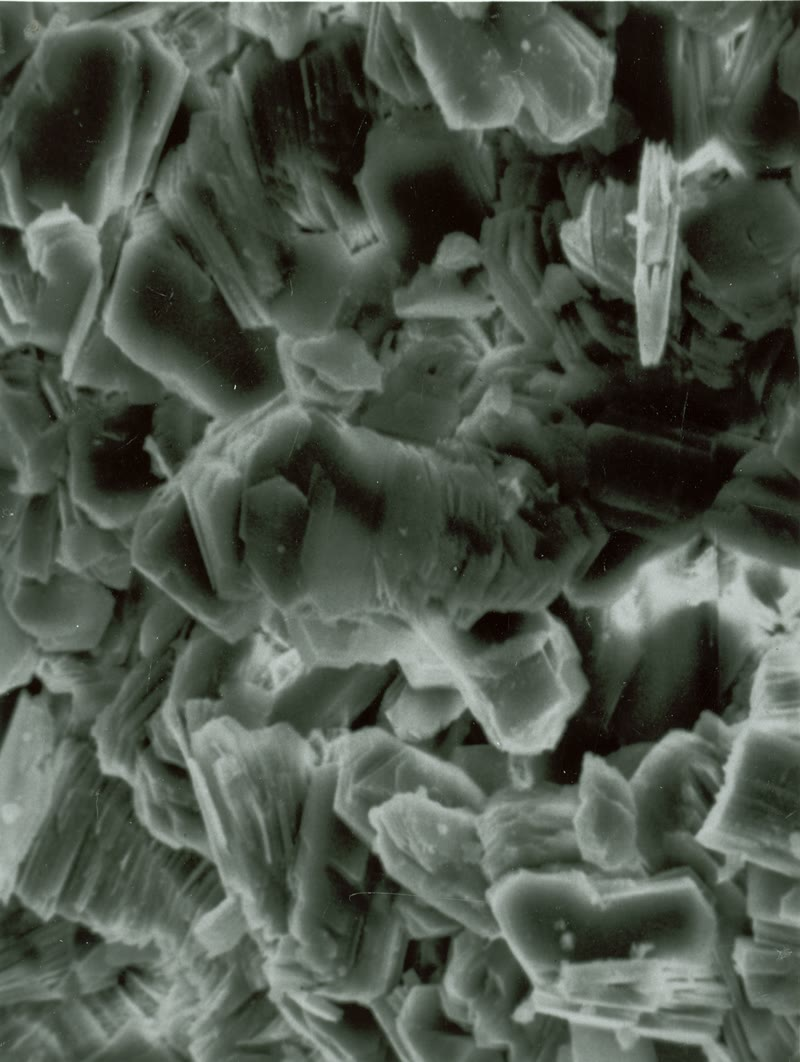
\includegraphics[width=\linewidth]{images/book3/b1-kaolinite-sem.jpg}

{\scriptsize उत्तरी अलास्का के एक बलुआ पत्थर के छिद्रों में उगे \omterm{def:b1:weathering-clays:clay-mineral}{कैओलिनाइट} को स्कैनिंग इलेक्ट्रॉन सूक्ष्मदर्शी से देखा गया: षट्भुजाकार पत्रों के ढेरों की पुस्तकें (आवर्धन लगभग 1340)। फ़ोटो: U.S. Geological Survey, सार्वजनिक क्षेत्र, विकिमीडिया कॉमन्स के माध्यम से।\par}
\end{minipage}
\end{omfigure}
% ledger: biscaye:1965, usgs:clay-settings, pedron:stages, commons:kaolinite-sem

\emph{\omterm{def:b1:weathering-clays:laterite}{लैटेराइट}।} जहाँ \omterm{def:b1:weathering-clays:hydrolysis}{जल-अपघटन} लंबे समय तक अपनी अंतिम मात्राओं तक पहुँचता है, परिच्छेद मोटा होता है और उसका शीर्ष हर उस चीज़ को सांद्रित करता है जो नहीं निकलती।

\begin{definition}[लैटेराइट]
\label{def:b1:weathering-clays:laterite}
एक \emph{लैटेराइट}\index{लैटेराइट} तीव्र और दीर्घ \omterm{def:b1:weathering-clays:hydrolysis}{जल-अपघटन} का लौह- और ऐल्युमिनियम-समृद्ध उत्पाद है, गर्म, आर्द्र जलवायु में: एक लाल से भूरा पदार्थ, मुलायम या कठोर, जो \omterm{def:b1:weathering-clays:clay-mineral}{कैओलिनाइट} और लौह-ऑक्साइडों तथा हाइड्रॉक्साइडों से बना है, \omterm{def:b1:weathering-clays:hydrolysis-degree}{ऐलिटीकरण} पहुँचने पर गिब्साइट के साथ, जिससे लगभग सारे क्षारीय और क्षारीय-मृदा धनायन और सिलिका का बहुत-सा भाग हटा दिया गया है।
\end{definition}
% ledger: formoso:laterite, buchanan:laterite

पर्याप्त गिब्साइट या बोएमाइट, ऐल्युमिनियम हाइड्रॉक्साइड, वाला \omterm{def:b1:weathering-clays:laterite}{लैटेराइट} एक बॉक्साइट है, जो नौ-दसवें ऐल्युमिनियम का अयस्क है: \omterm{def:b1:weathering-clays:hydrolysis-degree}{ऐलिटीकरण} वह चरण है जो अयस्क बनाता है। अधिकांश बॉक्साइट अवशेषी हैं, वह चट्टान जिससे ऐल्युमिना को छोड़कर सब कुछ निक्षालित हो गया है; गिब्साइट के बने अधिकांश उष्णकटिबंध में हैं, और उनमें से कई शायद अब भी बन रहे हैं।
% ledger: usgs:bauxite

\begin{history}[क्षेत्र से एक शब्द]
1807 में फ़्रांसिस बुकानन ने मलाबार, दक्षिणी प्रायद्वीप में यात्रा करते हुए एक ऐसी सामग्री का वर्णन किया जो गुहिकाओं से भरी थी और लोहे के लाल और पीले गेरुओं से समृद्ध थी, ग्रेनाइट पर बड़े पुंजों में फैली। ज़मीन से खोदने पर वह इतनी मुलायम थी कि चाकू से कट जाती थी, और निवासी उसे खंडों में गढ़ते थे; हवा में वह शीघ्र ही ईंट जितनी कठोर हो गई, और उसने जितनी भी ईंटें देखी थीं उनसे बेहतर टिकी। स्थानीय भाषाओं में उसे ईंट-पत्थर कहा जाता था; उसने \omterm{def:b1:weathering-clays:laterite}{लैटेराइट} नाम प्रस्तावित किया, जिसे भूविज्ञान ने उष्णकटिबंधीय अपक्षय के लाल उत्पादों के लिए रखा।
\end{history}
% ledger: buchanan:laterite

\section{सिलिकेट अपक्षय और कार्बन डाइऑक्साइड}\label{sec:b1:weathering-clays:co2}

\omterm{def:b1:weathering-clays:hydrolysis}{जल-अपघटन} के हाइड्रोजन आयन अधिकतर कार्बन डाइऑक्साइड से आते हैं, इसलिए उन्हें कार्बोनिक अम्ल के रूप में लिखना दिखाता है कि अपक्षय हवा के साथ क्या करता है। एक कैल्शियम सिलिकेट के लिए, सरलता के लिए \ce{CaSiO3} लिखा हुआ,
\[
  \ce{CaSiO3 + 2 CO2 + H2O -> Ca^2+ + 2 HCO3- + SiO2},
\]
और महासागर में, जहाँ जीव कैल्शियम कार्बोनेट के खोल बनाते हैं,
\[
  \ce{Ca^2+ + 2 HCO3- -> CaCO3 + CO2 + H2O}.
\]

\begin{proposition}[अपक्षय और कार्बन डाइऑक्साइड]\label{prop:b1:weathering-clays:co2}
(a) एक सिलिकेट का अपक्षय कार्बन डाइऑक्साइड के दो मोल का बाइकार्बोनेट में बदलकर उपभोग करता है, जो मुक्त किए गए कैल्शियम या मैग्नीशियम के हर मोल के लिए; जब कैल्शियम या मैग्नीशियम कार्बोनेट के रूप में अवक्षेपित होता है, तो दो में से एक वापस हवा में लौटता है, और एक मोल कार्बोनेट चट्टान के रूप में संचित होता है। (b) एक कार्बोनेट चट्टान का अपक्षय और उसके कार्बोनेट का फिर से अवक्षेपण कुछ भी संचित नहीं करता।
\end{proposition}

\begin{proof}
(a) दोनों ऊपर के समीकरणों को जोड़ने पर \ce{CaSiO3 + CO2 -> CaCO3 + SiO2} मिलता है: हर कैल्शियम के लिए एक \ce{CO2} हवा को सदा के लिए छोड़ता है; अकेला पहला समीकरण दिखाता है कि दो उपभुक्त होते हैं। मैग्नीशियम के लिए वही सही है, \ce{Mg^2+} के साथ, \ce{Ca^2+} के स्थान पर। (b) कैल्साइट का घुलना, \ce{CaCO3 + CO2 + H2O -> Ca^2+ + 2
HCO3-}, अवक्षेपण का ठीक विलोम है: दोनों का योग शून्य है।
\end{proof}

फ़ेल्डस्पार के साथ, कार्बोनिक अम्ल \cref{prop:b1:weathering-clays:feldspars} के हाइड्रोजन आयनों का स्थान लेता है: उपभुक्त हर \ce{H+} एक \ce{CO2} है जो \ce{HCO3-} बनती है। एक बेसाल्ट या गैब्रो का एनॉर्थाइट इस प्रकार \omterm{def:b1:weathering-clays:clay-mineral}{कैओलिनाइट} में बदलते हुए प्रति मोल दो मोल कार्बन डाइऑक्साइड उपभुक्त करता है,
\[
  \ce{CaAl2Si2O8 + 2 CO2 + 3 H2O -> Al2Si2O5(OH)4 + Ca^2+ + 2 HCO3-},
\]
और दीर्घकालिक रूप से एक संचित करता है। सोडियम और पोटैशियम समुद्र-तल पर कोई कार्बोनेट नहीं बनाते, और दीर्घकालिक संचयन मुक्त हुए कैल्शियम और मैग्नीशियम से गिना जाता है।

नदियाँ बाइकार्बोनेट को समुद्र तक ले जाती हैं, और उनकी रसायन-विज्ञान प्रवाह मापती है। विश्व की बड़ी नदियों की रसायन-विज्ञान से, महाद्वीपीय सिलिकेटों के अपक्षय द्वारा उपभुक्त कार्बन डाइऑक्साइड का अनुमान \num{11.7e12} से \qty{13.6e12}{mol} प्रति वर्ष लगाया गया है, लगभग 0.14 से 0.16 अरब टन कार्बन, जिसमें अकेले बेसाल्टों का अपक्षय 30 से \qty{35}{\percent} हिस्सा देता है। यह प्रवाह हवा, महासागरों और जीवित प्राणियों के बीच कार्बन के आदान-प्रदान की तुलना में छोटा है, पर वह उलटता नहीं: लाखों वर्षों में यही वह मुख्य तरीका है जिससे ज्वालामुखियों से आई कार्बन डाइऑक्साइड वायुमंडल छोड़ती है। क्योंकि अपक्षय गरम और आर्द्र होने पर तेज़ चलता है, वह हवा की कार्बन डाइऑक्साइड को जलवायु से बाँधता है, जो बदले में ग्रीनहाउस प्रभाव के माध्यम से कार्बन डाइऑक्साइड पर निर्भर है: एक ऋणात्मक प्रतिपुष्टि जो भूवैज्ञानिक काल में पृथ्वी के ताप को स्थिर रखती है, जिसका अध्ययन पुस्तक 4 में होता है।
% ledger: dessert:silicate-co2, whk:1981

\section{अभ्यास}

\begin{exercise}[$\star$]
\label{exo:b1:weathering-clays:1}
त्रिज्याएँ \ce{K+} \qty{1.38}{\angstrom}, \ce{Fe^2+} \qty{0.78}{\angstrom},
\ce{Fe^3+} \qty{0.645}{\angstrom} और \ce{Ti^4+} \qty{0.605}{\angstrom} लेकर, हर आयन का \omterm{def:b1:weathering-clays:ionic-potential}{आयनिक विभव} परिकलित कीजिए और उसका क्षेत्र बताइए। जलमग्न मिट्टी अपना लोहा क्यों खोती है, जबकि अच्छी तरह निकास वाली मिट्टी उसे रखती है?
% ledger: shannon:radii-b19
\end{exercise}

\begin{exercise}[$\star$]
\label{exo:b1:weathering-clays:2}
चार मृत्तिका-भिन्नों का अभिविन्यस्त माउंटों पर X-किरण विवर्तन किया जाता है। A: \SI{14}{\angstrom} पर एक शिखर, एथिलीन ग्लाइकॉल से \SI{17}{\angstrom} और \SI{400}{\celsius} तक तपाने से \SI{10}{\angstrom} तक खिसकता हुआ। B: \SI{7}{\angstrom} पर एक शिखर, ग्लाइकॉल से अपरिवर्तित, \SI{550}{\celsius} तक तपाने के बाद लुप्त। C: \SI{10}{\angstrom} पर एक शिखर जिसे कोई उपचार नहीं खिसकाता। D: \SI{14}{\angstrom} पर एक शिखर जिसे कोई उपचार नहीं खिसकाता। हर \omterm{def:b1:rock-forming-minerals:mineral}{खनिज} पहचानिए।
% ledger: usgs:clay-xrd
\end{exercise}

\begin{exercise}[$\star$]
\label{exo:b1:weathering-clays:3}
\cref{met:b1:weathering-clays:balance} से, ऑर्थोक्लेज़ \ce{KAlSi3O8} के \omterm{def:b1:weathering-clays:clay-mineral}{कैओलिनाइट} में \omterm{def:b1:weathering-clays:hydrolysis}{जल-अपघटन} का संतुलन कीजिए। उसके पोटैशियम और उसके सिलिकॉन का कितना भाग विलयन में निकलता है?
\end{exercise}

\begin{exercise}[$\star$]
\label{exo:b1:weathering-clays:4}
(a) \qty{0}{\celsius} पर \qty{10}{cm^3} जल कितना बर्फ़ का आयतन देता है? (b) किस ताप-परास में दरारों में बढ़ती बर्फ़ चट्टान को सबसे प्रभावी ढंग से तोड़ती है, और क्यों न हल्का और न कठोर पाला उतना ही अच्छा करता है? (c) \qty{1}{m} भुजा के एक ग्रेनाइट घन को पाले से \qty{1}{cm} भुजा वाले घनों में तोड़ा जाता है: उसका सतह-क्षेत्रफल किस गुणक से बढ़ा है?
% ledger: usgs:water-density, iapws:ice-density, wh85:frost
\end{exercise}

\begin{exercise}[$\star\star$]
\label{exo:b1:weathering-clays:5}
घनत्व \qty{2600}{kg.m^{-3}} के फ़ेल्डस्पार कणों की विशिष्ट सतह परिकलित कीजिए, जिन्हें घन मानकर, आकारों \qty{1}{cm}, \qty{1}{mm} और \qty{1}{\micro m} के लिए। कण का आकार \omterm{def:b1:weathering-clays:weathering}{रासायनिक अपक्षय} की दर के लिए इतना क्यों मायने रखता है, और \omterm{def:b1:weathering-clays:weathering}{भौतिक अपक्षय} \omterm{def:b1:weathering-clays:weathering}{रासायनिक अपक्षय} को क्यों तेज़ करता है?
\end{exercise}

\begin{exercise}[$\star\star$]
\label{exo:b1:weathering-clays:6}
एक टन एल्बाइट \ce{NaAlSi3O8} (\qty{262.22}{g.mol^{-1}}) \omterm{def:b1:weathering-clays:clay-mineral}{कैओलिनाइट} (\qty{258.16}{g.mol^{-1}}) में बदलता है। बने \omterm{def:b1:weathering-clays:clay-mineral}{कैओलिनाइट} का द्रव्यमान, निर्यातित सिलिका का द्रव्यमान, \ce{SiO2} (\qty{60.08}{g.mol^{-1}}) के रूप में गिना गया, और निर्यातित सोडियम का द्रव्यमान परिकलित कीजिए।
% ledger: webmineral:clays-b19, ciaaw:Na
\end{exercise}

\begin{exercise}[$\star\star$]
\label{exo:b1:weathering-clays:7}
एक ग्रेनाइट में द्रव्यमान से \qty{0.30}{\percent} \ce{TiO2}, \qty{3.5}{\percent}
\ce{Na2O}, \qty{72}{\percent} \ce{SiO2} और \qty{14}{\percent} \ce{Al2O3} है; उसकी सैप्रोलाइट में \qty{0.60}{\percent} \ce{TiO2}, \qty{0.35}{\percent}
\ce{Na2O}, \qty{60}{\percent} \ce{SiO2} और \qty{27}{\percent} \ce{Al2O3} है। टाइटेनियम को अचल मानकर, एक किलोग्राम ग्रेनाइट द्वारा छोड़ी गई सैप्रोलाइट का द्रव्यमान और सोडियम, सिलिकॉन तथा ऐल्युमिनियम का खोया भाग ज्ञात कीजिए। कौन-सी \omterm{def:b1:weathering-clays:hydrolysis}{जल-अपघटन} की मात्रा चल रही है?
\end{exercise}

\begin{exercise}[$\star\star$]
\label{exo:b1:weathering-clays:8}
\cref{prop:b1:weathering-clays:layer-charge} का उपयोग करके, पाइरोफ़िलाइट \ce{Al2Si4O10(OH)2} का परत-आवेश, \ce{KAl2(Si3Al)O10(OH)2} मस्कोवाइट का, उसके पोटैशियम के बिना, बेइडेलाइट परत \ce{Al2(Si_{3.5}Al_{0.5})O10(OH)2} का और एक मॉन्टमॉरिलोनाइट परत \ce{(Al_{1.67}Mg_{0.33})Si4O10(OH)2} का परिकलित कीजिए। उनमें से कौन फूल सकता है, और क्यों?
% ledger: webmineral:clays-b19
\end{exercise}

\begin{exercise}[$\star\star$]
\label{exo:b1:weathering-clays:9}
फ़ॉर्स्टेराइट \ce{Mg2SiO4} इस प्रकार अपक्षयित होता है:
\ce{Mg2SiO4 + 4 CO2 + 4 H2O -> 2 Mg^2+ + 4 HCO3- + H4SiO4}। (a) समीकरण जाँचिए। (b) एक टन फ़ॉर्स्टेराइट के लिए, उपभुक्त कार्बन डाइऑक्साइड और \cref{prop:b1:weathering-clays:co2} के अनुसार दीर्घकालिक रूप से संचित कार्बन डाइऑक्साइड परिकलित कीजिए। (c) एक टन कैल्साइट के लिए वही परिकलन क्या देता?
% ledger: ciaaw:Mg, ciaaw:Si, ciaaw:O, ciaaw:C
\end{exercise}

\begin{exercise}[$\star\star\star$]
\label{exo:b1:weathering-clays:10}
(a) किस त्रिज्या-परास के बीच आवेश 3 का एक आयन जल-अपघटन-उत्पाद है? (b) बोरॉन, \ce{B^3+}, की त्रिज्या \qty{0.27}{\angstrom} है: पानी में वह किस रूप में चलता है? (c) \ce{Mn^2+} की त्रिज्या \qty{0.83}{\angstrom} है, \ce{Mn^4+} की \qty{0.53}{\angstrom}। समझाइए कि मैंगनीज़ ऑक्साइड की काली परतें क्यों बनती हैं जहाँ ऑक्सीजन-दरिद्र स्रोत-जल हवा में निकलता है। (d) सिलिकॉन न पूरी तरह निक्षालित हो सकता है न पूरी तरह रखा जा सकता है: क्यों?
% ledger: shannon:radii-b19, nomad:goldschmidt
\end{exercise}

\begin{exercise}[$\star\star\star$]
\label{exo:b1:weathering-clays:11}
महाद्वीपीय सिलिकेटों का अपक्षय प्रति वर्ष \num{11.7e12} से \qty{13.6e12}{mol} कार्बन डाइऑक्साइड उपभुक्त करता है, जिसमें से \qty{4.08e12}{mol} बेसाल्टों से है। (a) परास को टन कार्बन और टन कार्बन डाइऑक्साइड प्रति वर्ष में बदलिए। (b) बेसाल्टों का हिस्सा कितना है? (c) यदि यह सारी कैल्शियम और मैग्नीशियम सिलिकेटों से आती, तो हर वर्ष दीर्घकालिक रूप से कितना कार्बन संचित होता? वास्तविक दीर्घकालिक आँकड़ा छोटा क्यों है?
% ledger: dessert:silicate-co2, ciaaw:C, ciaaw:O
\end{exercise}

\begin{exercise}[$\star\star\star$]
\label{exo:b1:weathering-clays:12}
तीन मृत्तिका-भिन्न, क्वार्ट्ज और आयरन ऑक्साइडों से मुक्त, विश्लेषित किए गए हैं (द्रव्यमान प्रतिशत): A, \ce{SiO2} \num{46.55} और \ce{Al2O3} \num{39.50}; B, \ce{SiO2} 60 और \ce{Al2O3} 25; C, \ce{SiO2} 2 और \ce{Al2O3} 63 (\ce{SiO2} \qty{60.08}{g.mol^{-1}}, \ce{Al2O3} \qty{101.96}{g.mol^{-1}})। हर एक का मोलर Si/Al अनुपात परिकलित कीजिए, वह \omterm{def:b1:weathering-clays:hydrolysis}{जल-अपघटन} की जो मात्रा दर्ज करता है उसे पहचानिए, और तीनों मिट्टियों को सबसे कम से सबसे तीव्र निक्षालन की एक रेखा पर रखिए।
% ledger: webmineral:clays-b19, pedron:stages, formoso:laterite
\end{exercise}

\section{समस्या: ग्रेनाइट से मृत्तिका तक}

\begin{problem}[{सप्ताहांत समस्या --- एक ग्रेनाइट और एक गैब्रो के फ़ेल्डस्पार, संतुलित अभिक्रियाओं से लेकर उस कार्बन डाइऑक्साइड तक जो एक नदी बहा ले जाती है}]
\label{pb:b1:weathering-clays:1}
% values: calc/ch19.py; the river is invented (its numbers are of a realistic order)
फ़ेल्डस्पार एल्बाइट \ce{NaAlSi3O8} (\qty{262.22}{g.mol^{-1}}, घनत्व \qty{2.62}{g.cm^{-3}}) और एनॉर्थाइट \ce{CaAl2Si2O8} (\qty{278.20}{g.mol^{-1}}, घनत्व \qty{2.75}{g.cm^{-3}}) हैं। \omterm{def:b1:weathering-clays:clay-mineral}{कैओलिनाइट} \ce{Al2Si2O5(OH)4} का मोलर द्रव्यमान \qty{258.16}{g.mol^{-1}} और घनत्व \qty{2.6}{g.cm^{-3}} है; गिब्साइट \ce{Al(OH)3}, \qty{78.00}{g.mol^{-1}}। \ce{SiO2} के लिए \qty{60.08}{g.mol^{-1}}, \ce{CO2} के लिए \qty{44.01}{g.mol^{-1}}, \ce{HCO3-} के लिए \qty{61.02}{g.mol^{-1}}, Na के लिए \num{22.99} और Ca के लिए \qty{40.08}{g.mol^{-1}} लीजिए।
% ledger: hom:albite, hom:anorthite, webmineral:clays-b19, ciaaw:Na, ciaaw:Ca, ciaaw:C, ciaaw:O, ciaaw:H

\medskip
\noindent\textbf{भाग I --- अभिक्रियाएँ।}
\begin{enumerate}
  \item एल्बाइट के \omterm{def:b1:weathering-clays:clay-mineral}{कैओलिनाइट} में \omterm{def:b1:weathering-clays:hydrolysis}{जल-अपघटन} का संतुलन कीजिए।
  \item एनॉर्थाइट के \omterm{def:b1:weathering-clays:clay-mineral}{कैओलिनाइट} में \omterm{def:b1:weathering-clays:hydrolysis}{जल-अपघटन} का संतुलन कीजिए। उसके बारे में क्या विशेष है?
  \item एनॉर्थाइट के गिब्साइट में \omterm{def:b1:weathering-clays:hydrolysis}{जल-अपघटन} का संतुलन कीजिए।
  \item एल्बाइट के बेइडेलाइट \ce{Na_{0.5}Al2(Si_{3.5}Al_{0.5})O10(OH)2} में \omterm{def:b1:weathering-clays:hydrolysis}{जल-अपघटन} का संतुलन कीजिए, और हाइड्रोजन जाँचिए।
  \item पहली दो अभिक्रियाओं को हाइड्रोजन आयनों के स्रोत के रूप में कार्बोनिक अम्ल के साथ फिर से लिखिए: \ce{CO2 + H2O -> H+ + HCO3-}।
  \item इनमें से कौन-सी अभिक्रियाएँ \omterm{def:b1:weathering-clays:hydrolysis-degree}{द्वि-सिऐलिटीकरण}, \omterm{def:b1:weathering-clays:hydrolysis-degree}{एक-सिऐलिटीकरण} और \omterm{def:b1:weathering-clays:hydrolysis-degree}{ऐलिटीकरण} हैं?
\end{enumerate}

\medskip
\noindent\textbf{भाग II --- क्या रुकता है, क्या निकलता है।}
\begin{enumerate}[resume]
  \item एक टन एल्बाइट और एक टन एनॉर्थाइट में कितने मोल हैं?
  \item हर एक से बने \omterm{def:b1:weathering-clays:clay-mineral}{कैओलिनाइट} का द्रव्यमान परिकलित कीजिए।
  \item विलयन में निर्यातित सिलिका (\ce{SiO2} के रूप में), सोडियम और कैल्शियम के द्रव्यमान परिकलित कीजिए।
  \item हर एक टन फ़ेल्डस्पार और उससे बने \omterm{def:b1:weathering-clays:clay-mineral}{कैओलिनाइट} का आयतन परिकलित कीजिए। ठोस का आयतन किस भिन्न से सिकुड़ता है?
  \item सैप्रोलाइट उस चट्टान का आकार रखता है जिसे वह बदलती है। एल्बाइट से समृद्ध एक अपक्षीकृत ग्रेनाइट में छूटी जगह क्या भरता है? एनॉर्थाइट से समृद्ध एक अपक्षीकृत गैब्रो क्यों सघन रहता है?
  \item आयनिक-विभव आरेख से समझाइए कि दोनों फ़ेल्डस्पारों के कौन-से तत्व निकलते हैं और कौन-से रुकते हैं।
\end{enumerate}

\medskip
\noindent\textbf{भाग III --- कार्बन डाइऑक्साइड।}
\begin{enumerate}[resume]
  \item जब एक टन एल्बाइट \omterm{def:b1:weathering-clays:clay-mineral}{कैओलिनाइट} में बदलता है, तो कितने मोल, और कितने किलोग्राम, कार्बन डाइऑक्साइड उपभुक्त होते हैं?
  \item एक टन एनॉर्थाइट के लिए वही प्रश्न।
  \item एनॉर्थाइट द्वारा कितने द्रव्यमान का बाइकार्बोनेट निर्यात होता है?
  \item इस बाइकार्बोनेट का महासागर में क्या होता है? उपभुक्त कार्बन डाइऑक्साइड का कितना भाग हवा में लौटता है?
  \item एल्बाइट के सोडियम के लिए दीर्घकालिक संचयन क्यों नहीं गिना जाता?
  \item एक टन कैल्साइट के घुलने और उसके बाद उसके अवक्षेपण से तुलना कीजिए।
\end{enumerate}

\medskip
\noindent\textbf{भाग IV --- एक नदी।}
\begin{enumerate}[resume]
  \item एक नदी \qty{50000}{km^2} ग्रेनाइट और नाइस को निकालती है, जिसका माध्य निस्सरण \qty{200}{m^3.s^{-1}} है; सिलिकेट अपक्षय से वह जो बाइकार्बोनेट ले जाती है वह \qty{0.3}{mmol.L^{-1}} है। इस बाइकार्बोनेट का वार्षिक प्रवाह, मोलों में, और प्रति वर्ग किलोमीटर, परिकलित कीजिए।
  \item इसे उन एनॉर्थाइट के मोलों के रूप में व्यक्त कीजिए जिनका \omterm{def:b1:weathering-clays:clay-mineral}{कैओलिनाइट} में अपक्षय इसे आपूर्ति करेगा, फिर एनॉर्थाइट के टनों में प्रति वर्ष और प्रति वर्ग किलोमीटर।
  \item यदि चट्टान में \qty{20}{\percent} एनॉर्थाइट के समतुल्य है और घनत्व \qty{2700}{kg.m^{-3}} है, तो ताज़ी चट्टान किस दर से, मीटर प्रति दस लाख वर्ष में, उपभुक्त हो रही है?
  \item यह नदी हर वर्ष हवा से कितनी कार्बन डाइऑक्साइड सदा के लिए हटाती है?
  \item प्रश्न 21 की दर भू-पृष्ठ के नीचे खिसकने के लिए निचली सीमा क्यों है?
  \item एक टन एनॉर्थाइट के अपक्षय से कितनी कार्बन डाइऑक्साइड सदा के लिए नीचे खींची जाती है, तीन अंकों तक, किलोग्राम में?
\end{enumerate}
\end{problem}
